\documentclass{beamer}


\author{Tina Dong}

\usetheme{metropolis}           
\title{DevClub: MQ and PUB/SUB }
\date{\today}

\begin{document}
\maketitle

\begin{frame}{Topics: Today's Topics}
    \begin{itemize}
        \item Basic Pattern
        \item i love sweet because 
        \begin{itemize}
            \item she is pretty
            \item she is smart
        \end{itemize}
        \item Guarantee of Message Passing
        \item NATS Introduction
        \item Real Case: Usage In PTM LeaderBoard
    \end{itemize}
\end{frame}

\begin{frame}{Basic Pattern: Message Queue}
    Both \textbf{Message Queue} and \textbf{PUB/Sub Broker} are about passing 
    \textbf{ephemeral} messages among endpoints.

    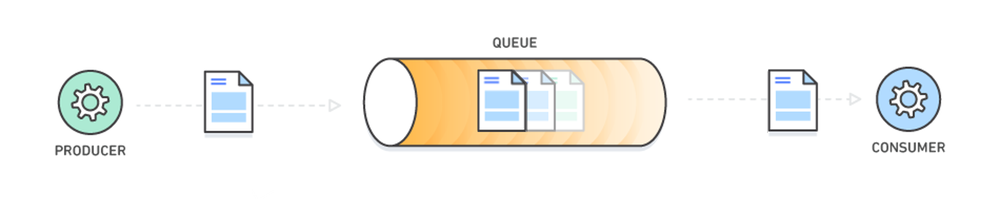
\includegraphics[width=\textwidth]{assets/mq.png}
    A \textbf{message queue} is a form of asynchronous service-to-service 
    communication used in serverless and microservices architectures.
\end{frame}

\begin{frame}{Basic Pattern: Pub/Sub Broker}
    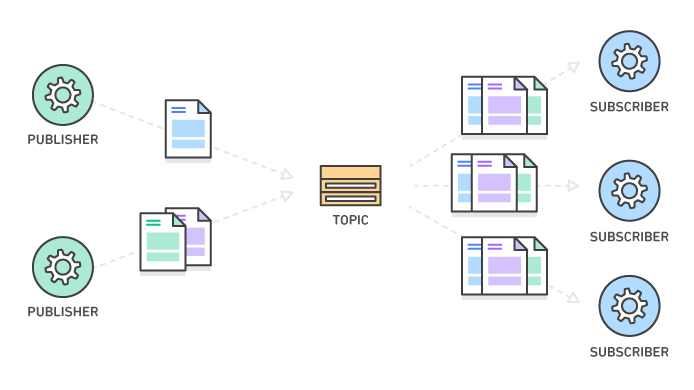
\includegraphics[width=\textwidth]{assets/pubsub.png}
    A \textbf{Publish/Subscribe} broker is also a form of communication middleware, but with different 
    message passing semantics.
\end{frame}

\begin{frame}{Common Problems:  Guarantee of Delivery}
    In most cases, we should care about the order and reliability of message passing.
    \\
    So, It is natural to ask these question when choosing middlewares.
    \begin{itemize}
        \item Does the Queue/Broker offer any guarantee of message ordering?
        \item Does Queue/Broker guarantee message delivery?
    \end{itemize}
\end{frame}

\begin{frame}{NATS Introduction: Overview}

    
\includegraphics[width=0.1\textwidth]{assets/NATSLogo.png}
    
\includegraphics[width=0.2\textwidth]{assets/CNCF.jpeg}
    Find more information \href{https://docs.nats.io}{Here}
    \\
    Quick Facts:
    \begin{itemize}
        \item CNCF Incubating Project.
        \item Various Delivary Guarantee: at least once, exactly once, at most once.
        \item Per-Publisher Order.
        \item Support Message replay/redelivery.
        \item Quick Deployment.
    \end{itemize}
\end{frame}

\begin{frame}{NATS: Subject Based Message}
    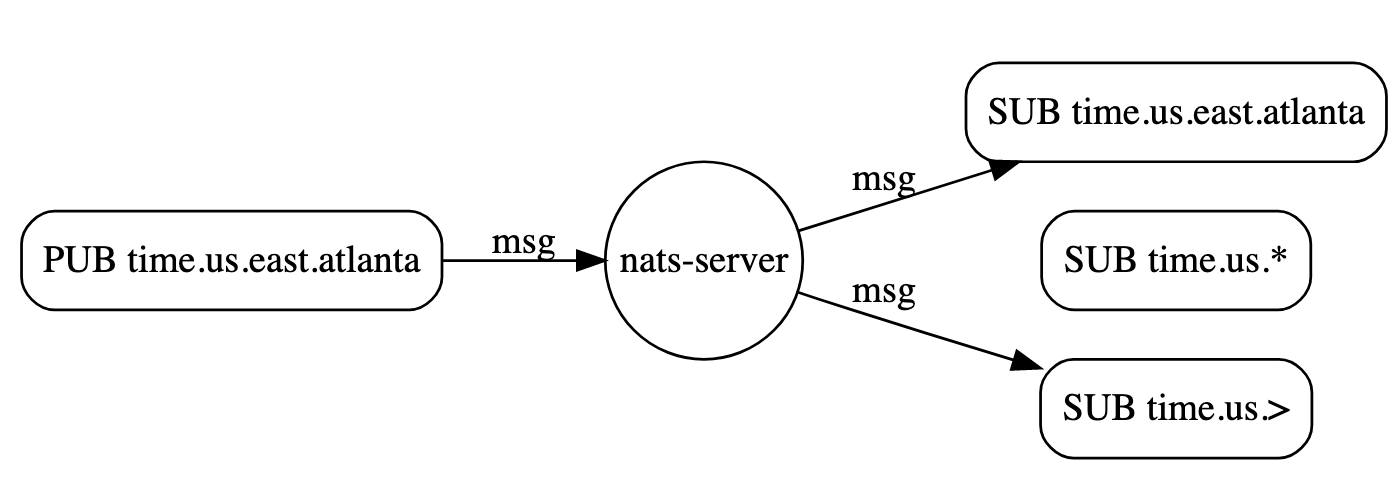
\includegraphics[width=\textwidth]{assets/Subject.png}
    \begin{itemize}
        \item $>$ and \textbf{*}
        \item mixed wildcard is supported
    \end{itemize}
\end{frame}

\begin{frame}{NATS: Queue Group}
    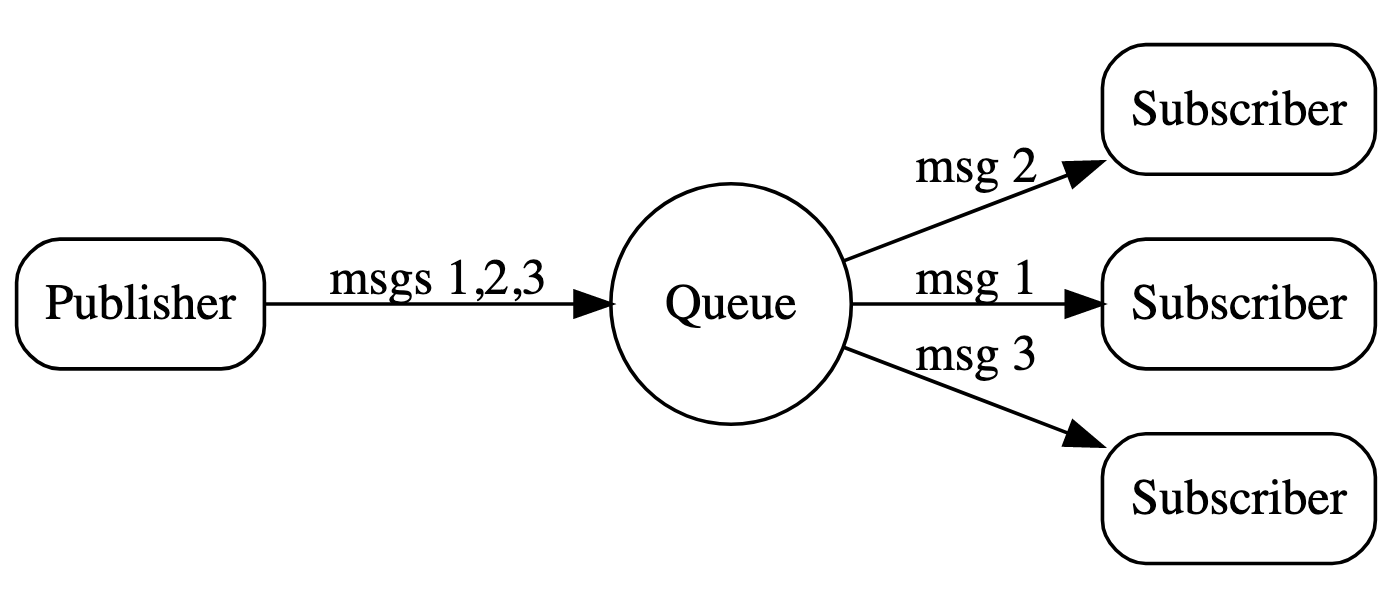
\includegraphics[width=\textwidth]{assets/MessageQueue.png}
    \begin{itemize}
        \item Besides The Subject Name, NATS also supports Queue name.
        \item Different Subscribers sharing the same Subject and Queue Name form a \textbf{Queue Group}.
        \item Mes.sage only passed to Queue Groups.
    \end{itemize}
\end{frame}

\begin{frame}{NATS: Request and Reply}
    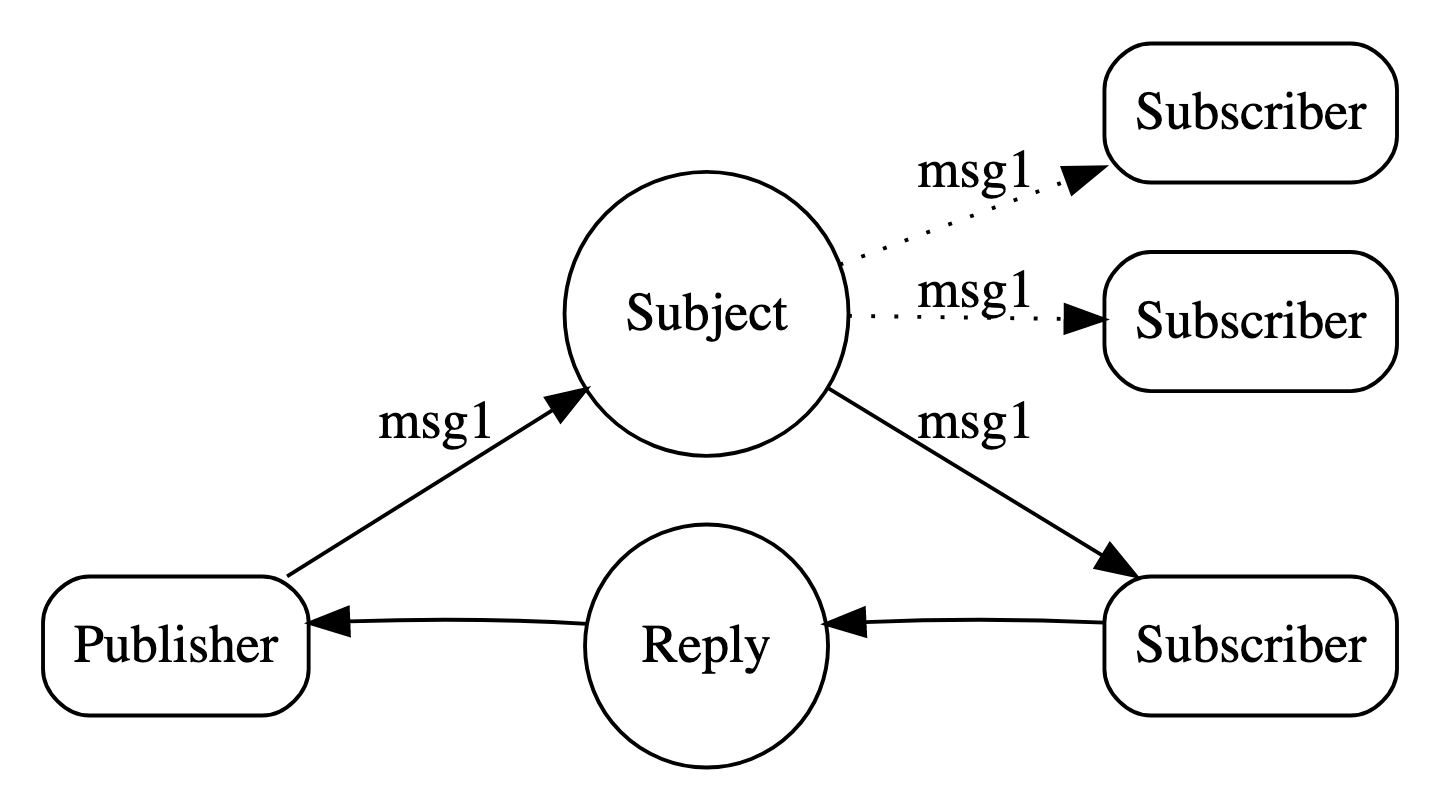
\includegraphics[width=\textwidth]{assets/Req.png}
    \begin{itemize}
        \item The latest NATS support websocket.
        \item This feature is good for Long Running Task.
    \end{itemize}
\end{frame}

\begin{frame}{Real Case: Usage In PTM LeaderBoard}
    \href{http://localhost:3000}{PTM-Leaderboard}
\end{frame}


\end{document}